\documentclass[main.tex]{subfiles}

\begin{document}

\section{A5 Stapelspeicher}
Sie wollen eine parametrisierte Klasse Stack für einen Stapelspeicher mit generischem Datentyp \texttt{TElement} für die Elemente implementieren. Für den Klassenparameter sollen alle Referenztypen erlaubt sein. Die Klasse soll die schreibgeschützten Attribute Capacity für die maximale Anzahl der Elemente und Count für die tatsächliche Anzahl der Elemente besitzen, beides vom Datentyp Integer.
Die Kapazität soll über den Konstruktor gesetzt werden können und ist immer mindestens 2.

Die möglichen Zustände des Stacks sind:
\begin{itemize}
    \item Empty: der Stapelspeicher enthält keine Elemente
    \item Filled: der Stapelspeicher enthält Elemente und kann noch neue Elemente aufnehmen
    \item Full: der Stapelspeicher ist voll und kann keine neuen Elemente mehr aufnehmen
\end{itemize}

Die Klasse hat die folgenden öffentlichen Operationen:
\begin{itemize}
    \item Push: lege das übergebene Element (vom Datentyp \texttt{TElement}) auf dem Stapelspeicher ab, wenn dieser noch nicht voll ist; ansonsten passiert nichts
    \item Pop: wenn der Stapelspeicher Elemente enthält, dann liefere das oberste Element zurück und entferne es vom Stapel; ansonsten wird NULL zurückgeliefert
    \item Peek: wenn der Stapelspeicher Elemente enthält, dann liefere das oberste Element zurück, ohne es vom Stapel zu nehmen; ansonsten wird NULL zurückgeliefert
\end{itemize}

Modellieren Sie die Klasse Stack als UML-Klassendiagramm und alle Zustandsübergänge als UML-Zustandsdiagramm. Nutzen Sie bei den Transitionen Call Events, Guards und Effects.

\subsection{Lösung 5}
\begin{figure}[h!]
    \makebox[\textwidth][c]{
        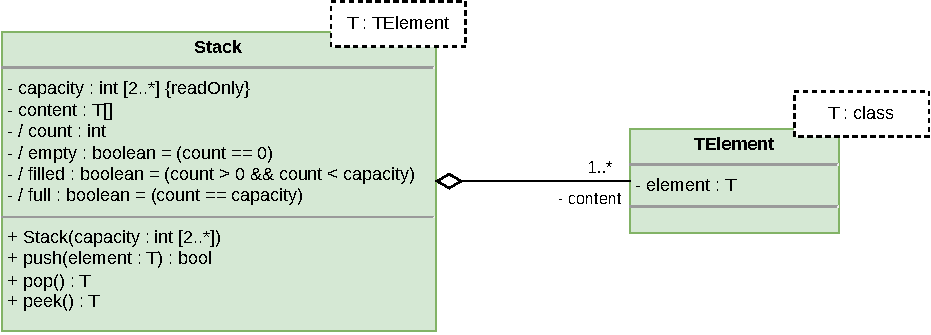
\includegraphics[width=1\linewidth]{h04_A5-Seite-1.drawio.pdf}
    }
    \caption{Klassendiagramm}
    \label{fig:lgs5a}
\end{figure}

\begin{figure}[h!]
    \makebox[\textwidth][c]{
        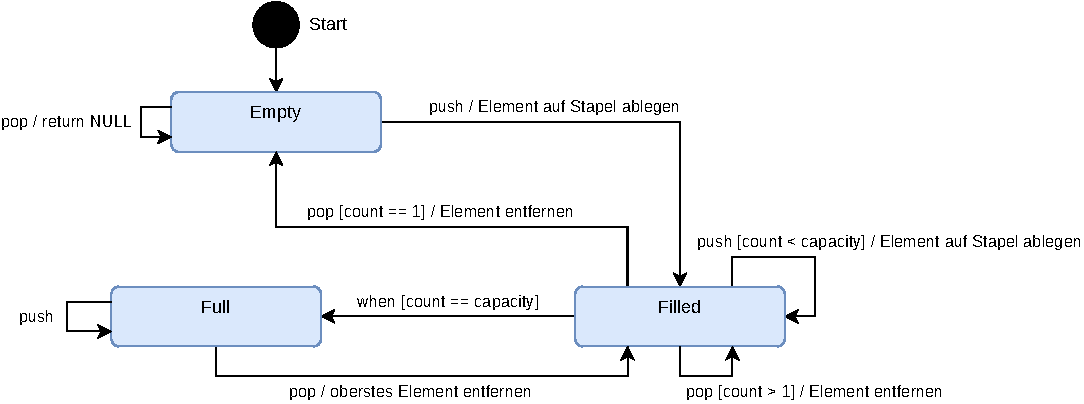
\includegraphics[width=1\linewidth]{h04_A5-Seite-2.drawio.pdf}
    }
    \caption{Zustandsdiagramm}
    \label{fig:lgs5b}
\end{figure}


\end{document}
